\section{RESULTADOS E DISCUSSÕES}

É imprescindível que a sociedade avance cada vez mais tecnologicamente. Porem esses avanços  podem trazer conflitos para a sociedade. A forma como a sociedade interage com essa novas tecnologias podem trazer benefícios ou maléficos para o meio. Em alguns desses casos o impacto pode ser percebido de diferentes formas,que variam de acordo com os valores morais dos indivíduos que a utilizam. 

A partir do conhecimento dos danos que as tecnologias podem gerar é de responsabilidade dos desenvolvedores tomarem medidas para minimizar ou evitar problemas nos desenvolvimento de novas tecnologias.

Outra forma que a robótica se relaciona com ética é através de robôs que passam por dilemas éticos em suas tomadas de decisão. Uma das soluções para esse problema é gerar algoritmos que seguem ordens de acordo com nossos valores éticos, outra solução é desenvolver maquinas que são capazes de ter raciocínio ético.

\subsection{Como questões éticos impactam no desenvolvimento de tecnologias}


\subsubsection{Tecnologias voltadas para o âmbito organizacional}

Com o avanço tecnológico as empresas certamente vão querer utilizar essas tecnologias para aumentar sua produtividade e melhorar sua produção. Com isso surgem investimentos na area de automação industrial \cite{Industri87:online}, mas também no quesito de gerenciamento de pessoas. Assim surgem novas tecnologias que visam aumentar essa produtividade.

Porém, como mostrado em \cite{Telkamp2022} o uso de inteligencia artificial para monitorar os empregados gera questionamentos éticos acerca dessas praticas gerarem abuso. A criação de sistemas que monitoram empregados ja foi aplicado pela \textit{Amazon}, mas não faltam relatos de que essas praticas são abusivas para com os empregados \cite{jef:online} \cite{Amazon:online}. 

\subsubsection{Tecnologias com capacidade de previsão}

No estudo realizado pela Universidade de Chicago é utilizado o machine learning para prever, através de areas de incidência, crimes futuros \cite{rotaru2021precise}. Embora realizar a previsão de crimes seja bastante positivo para a sociedade outros problemas podem ser gerados. Para melhorar o sistema de previsão o governo pode coletar os seus dados pessoais ferindo sua privacidade.


\subsection{Maquinas que tomam decisões éticas}

Devido ao uso de inteligencia artificial e a crescente automação das maquinas, os dispositivos são cada vez mais responsáveis por uma maior tomada de decisões. Porem essa tomadas de decisões podem carregar consigo um forte aspecto moral. Como em dilemas com carros autônomos, ou em triagem de hospitais. Assim as maquinas precisam ter uma base moral nelas para realizar a tomada de decisões.

A necessidade de analisar o pensamento ético de maquinas surge quando tomadas de decisões de robôs com alto nível de autonomia podem gerar impactos negativos na vida humana. Uma das formas pensadas para solucionar esse tipo de problema seria treinar inteligencias artificiais com capacidade de pensamento ético.

Como mostrado por \cite{vanWynsberghe2019719} só por um robô estar em uma situação de conflito ético não é necessário que ele seja uma maquina moral. Essa questão pode ser simplesmente resolvida com algoritmos sem necessidade de discernimento ético. Com isso então pode-se separar a ética na robótica em dois principais ramos: aqueles que realmente necessitem de maquinas morais, ou aqueles que precisam apenas de algoritmos que trabalhem com ética.

O problemas de se trabalhar com valores morais é eles variam de pessoa para pessoa. Sendo assim comunidades ou grupos podem perceber medidas de forma diferente de outros. No caso de um modelo de AI que faça escolhas sobre o que um carro vai bater caso os freios falhem as pessoas podem perceber que os mais novos devem ser priorizados. Enquanto outras pessoas podem achar que isso é uma forma de descriminação e que essa escolha deve ser aleatória \cite{Telkamp2022}.

De acordo com a Moral Fundations Theory \cite{GRAHAM201355} as pessoas diferem entre si em seis principais fundações morais: cuidado ou prejuízo, honestidade ou desonestidade, lealdade ou traição, autoridade ou subversão, pureza ou degeneração e liberdade ou opressão.

\begin{table}
    \centering
    \begin{tabular}{ m{6cm} m{8cm}}
        \hline
        AI issues & Conflicting concerns based on moral foundation \\
        \hline

        \multirow[m]{5}{6cm}{An AI system’s decision of whom or what to crash into when the brakes fail on a self driving car}
        
        & Authority—Save respected members or leaders of the community over those who are at the bottom of the hierarchy. Prioritize law-abiding citizens over those who are breaking the law (e.g., someone jaywalking) \newline \\ 

        & Care—Prioritize children first and attempt to reduce the overall number of people injured or killed \newline\\ 

        & Fairness—Do not consider characteristics such as age or status and instead randomly pick the outcome \newline \\

        & Loyalty—Protect the vehicle’s passengers at all costs because one family member or friend is more important than several out-group members \newline \\

        & Purity—A self-driving car in and of itself is morally wrong because human judgment is sacred \\

        \hline
    \end{tabular}
    \caption{AI issues involving moral foundations \cite{Telkamp2022}}
    \label{table:cars}
\end{table}

Essas variações podem gerar conflitos acerca de quais decisões tomar em determinado problema moral. Como mostrado na tabela \ref{table:cars} as diferentes visões de mundo entram em conflito dentro de um mesmo dilema moral. Assim é importante levar em consideração como a população vai receber certas decisões de algoritmos.

Conhecendo das diferentes percepções de mundo é interessante estuda-las para saber como a maioria das pessoas a percebem. Desse modo, foi feito um estudo onde se perguntava ao publico qual seria a melhor decisão a ser tomada no caso do carro autônomo.

\begin{figure}[h!]
    \centering
    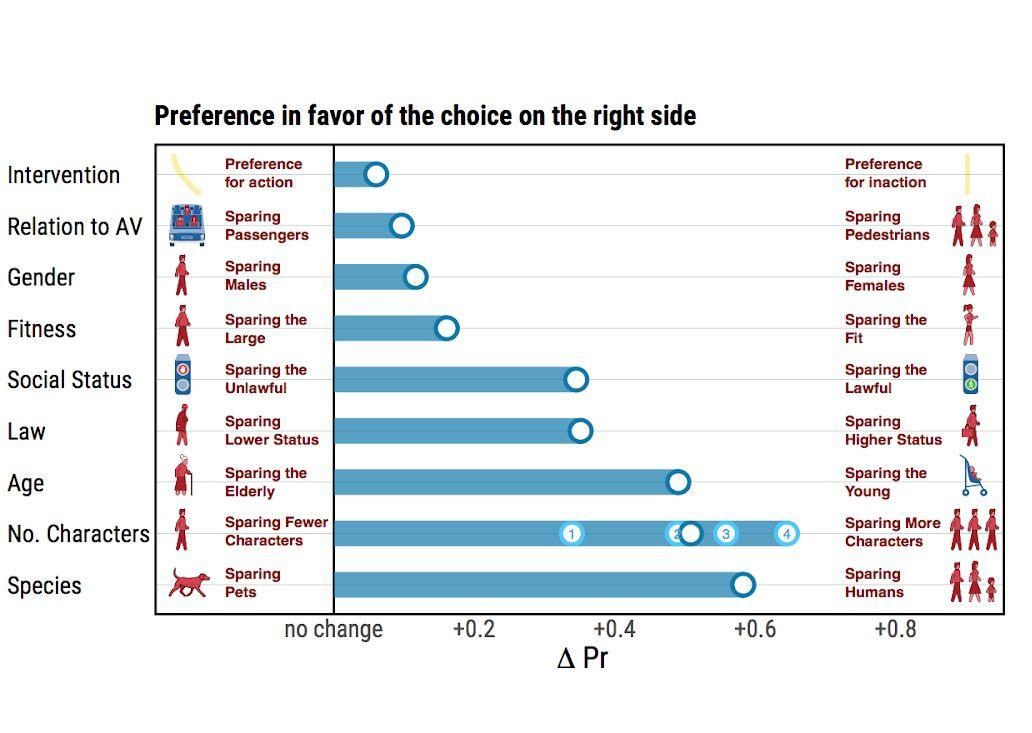
\includegraphics[width=15cm]{source/pictures/moral-machine.jpeg}
    \caption{Resultados do experimento da maquina moral \cite{Awad201859}}
    \label{fig:moral}
\end{figure}

Com o estudo perguntando pessoas de cerca de 130 paises diferentes se chegou ao resultado mostrado na figura \ref{fig:moral}. A partir desses resultados pode-se observar quais as preferencias da maioria em relação aos trade-offs comuns nesse tipo de situação.

Depois dessas conclusões pode-se usar os dados obtidos para modelar inteligencias artificiais que sigam esse tipo de informação. Um trabalho utilizando essa mesma base de dados conseguiu desenvolver uma inteligencia artificial que toma decisões com base nos valores morais ja estabelecidos

\begin{figure}[h!]
    \centering
    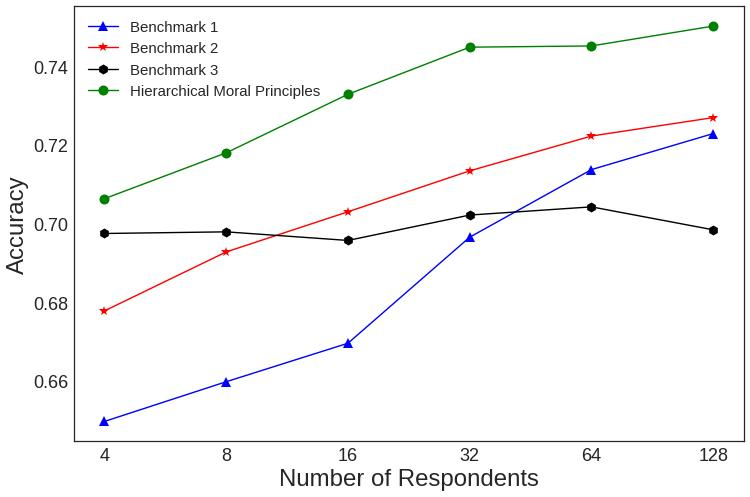
\includegraphics[width=7cm]{source/pictures/grapic.jpeg}
    \caption{Comparação dos resultados do modelo com pesquisas \cite{Kim2018197}}
    \label{fig:grapic}
\end{figure}

Na figura \ref{fig:grapic} mostra o resultado dos dados obtidos pelo dispositivo artificial comparado a diferentes tamanhos de bancos de dados. Mostrando como o modelo de predição possui uma boa acurácia.
